\begin{longtable} { | c | p{12cm} | c | } 
\hline
	ID 	&	Issues	&		 Es. hours \\\hline
	34 	&	Choices in Sequences	&	16 hours \\\hline
\caption{Issue ID 34}
\label{tab:spr3_choicesinsequences}
\end{longtable}

As choices was now able to add in sequences, we needed some way to display and editing choices. \note{INDSÆT BILLEDE AF DIALOGBOX MED CHOICE} The group `Lifestories' had a way to show and display choices, but we found that the theme of their dialog box did not fit well into Sekvens. We wanted to keep editing consistent within the application itself, so we chose to use the same \ct{ViewGroups} to have them completely similar. We created a fully customizable dialog box and created a new \ct{SequenceViewGroup} within it. The following figures (figure \ref{fig:SequenceViewGroup} and figure \ref{fig:choiceDialog}) shows how the code is written and how portrayed in figure \ref{fig:magicshit}

\begin{figure}
\centering
\begin{minipage}{.90\textwidth}
\centering
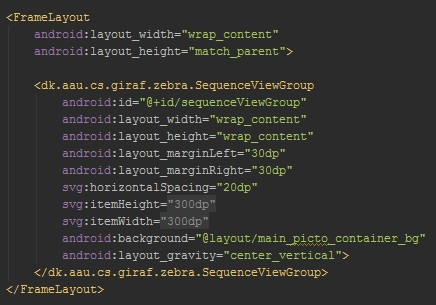
\includegraphics{Pics/Sprint3/SequenceViewGroup.jpg}
\caption{the XML code scrolling grid view we used in sequenceActivity as well}
\label{fig:SequenceViewGroup}
\end{minipage}\hfill
\begin{minipage}{.90\textwidth}
\centering
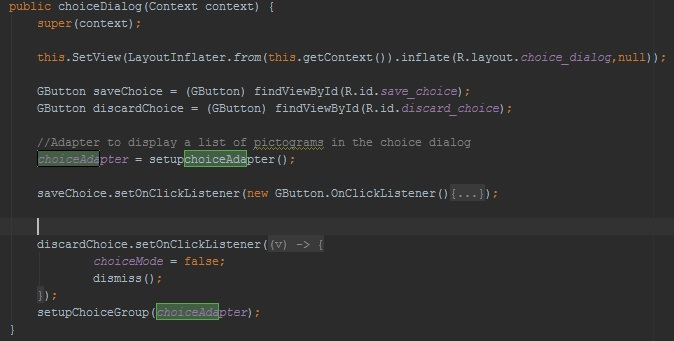
\includegraphics{Pics/Sprint3/ChoiceDialog.jpg}
\caption{The implementation of choiceDialog}
\label{fig:choiceDialog}
\end{minipage}\hfill
\begin{minipage}{.90\textwidth}
\centering
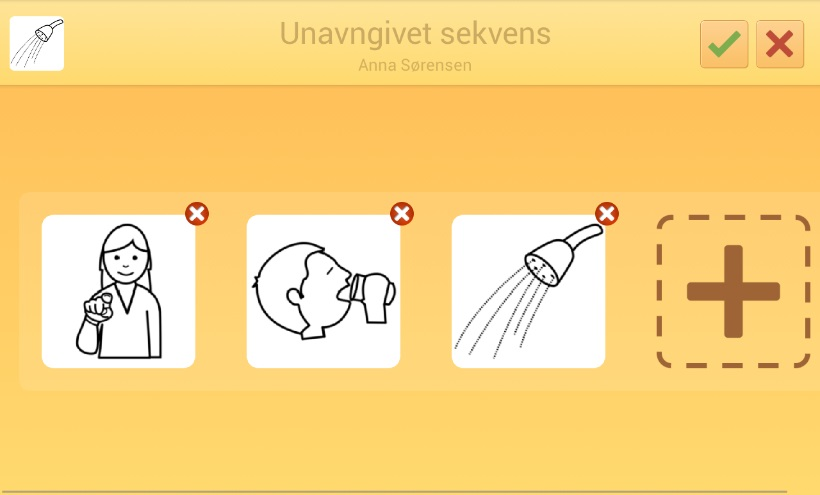
\includegraphics[width=14cm]{Pics/Sprint3/EditModeCropped.jpg}
\caption{THISISAPLACEHOLDER}
\label{fig:magicshit}
\end{minipage}
\end{figure}
